\documentclass[12pt,a4paper]{article}

%--------------------------------
% PAQUETES
%--------------------------------
\usepackage[spanish]{babel}
\usepackage[utf8]{inputenc}
\usepackage[T1]{fontenc}
\usepackage{geometry}
\usepackage{graphicx}
\usepackage{float}
\usepackage{amsmath}
\usepackage{siunitx}
\usepackage{hyperref}

\DeclareSIUnit{\V}{\volt}
\DeclareSIUnit{\A}{\ampere}
\DeclareSIUnit{\W}{\watt}
\DeclareSIUnit{\Hz}{\hertz}
\DeclareSIUnit{\mA}{\milli\ampere}
\DeclareSIUnit{\uA}{\micro\ampere}
\DeclareSIUnit{\F}{\farad}
\DeclareSIUnit{\k}{\kilo}
\DeclareSIUnit{\Omega}{\ohm}
\DeclareSIUnit{\mV}{\milli\volt}
\DeclareSIUnit{\dB}{\decibel}
\DeclareSIUnit{\celsius}{\degreeCelsius}
\DeclareSIUnit{\Ce}{\degreeCelsius}

\geometry{margin=2.5cm}

%--------------------------------
% DATOS DEL INFORME
%--------------------------------

\begin{document}

%--------------------------------
% PORTADA
%--------------------------------
\pagenumbering{gobble}
\begin{titlepage}
    \centering

    {\scshape\LARGE Universidad Tecnológica Nacional \par}
    \vspace{0.3cm}
    {\scshape\Large Facultad Regional Córdoba \par}
    \vspace{1.5cm}

    {\scshape\Large Electrónica Aplicada I \par}
    \vspace{2cm}

    {\Huge\bfseries Trabajo Práctico N°2 \par}
    \vspace{0.5cm}
    {\LARGE Fuente de Alimentación \par}

    \vspace{2cm}

    \begin{flushleft}
    \textbf{Integrantes:} \\
    Cortesini Pérez, Luciano Tomás -- 402719 \\
    Moreyra, Iván Agustín -- 413687 \\
    Pedregoza, Juan Ignacio  -- 408644 \\

    \vspace{0.5cm}

    \textbf{Curso:} 3R\_4 \\
    %\textbf{Grupo:} 02 \\
    \textbf{Docente:} Ing. Pablo Miklosa ; Dr. Ing. Guillermo Riva  \\
    \textbf{Año:} 2026 \\
    \end{flushleft}

    \vfill

\end{titlepage}
\thispagestyle{empty}

\vspace{1cm}

\tableofcontents
\newpage
\pagenumbering{arabic}

%--------------------------------
\section{Introducción}
%--------------------------------
El presente trabajo práctico aborda el diseño, análisis teórico y verificación experimental de una fuente de alimentación
regulada lineal. Se analiza la etapa de rectificación de onda completa mediante un transformador con derivación central
(toma media), el filtrado capacitivo para la reducción del rizado y la regulación de tensión de salida mediante el
circuito integrado LM317. Asimismo, se evalúan experimentalmente los parámetros característicos de regulación de línea,
regulación de carga y el comportamiento térmico del regulador bajo condiciones de carga máxima.

\vspace{0.5cm}

\section{Circuito esquemático}

\begin{figure}[H]
    \centering
    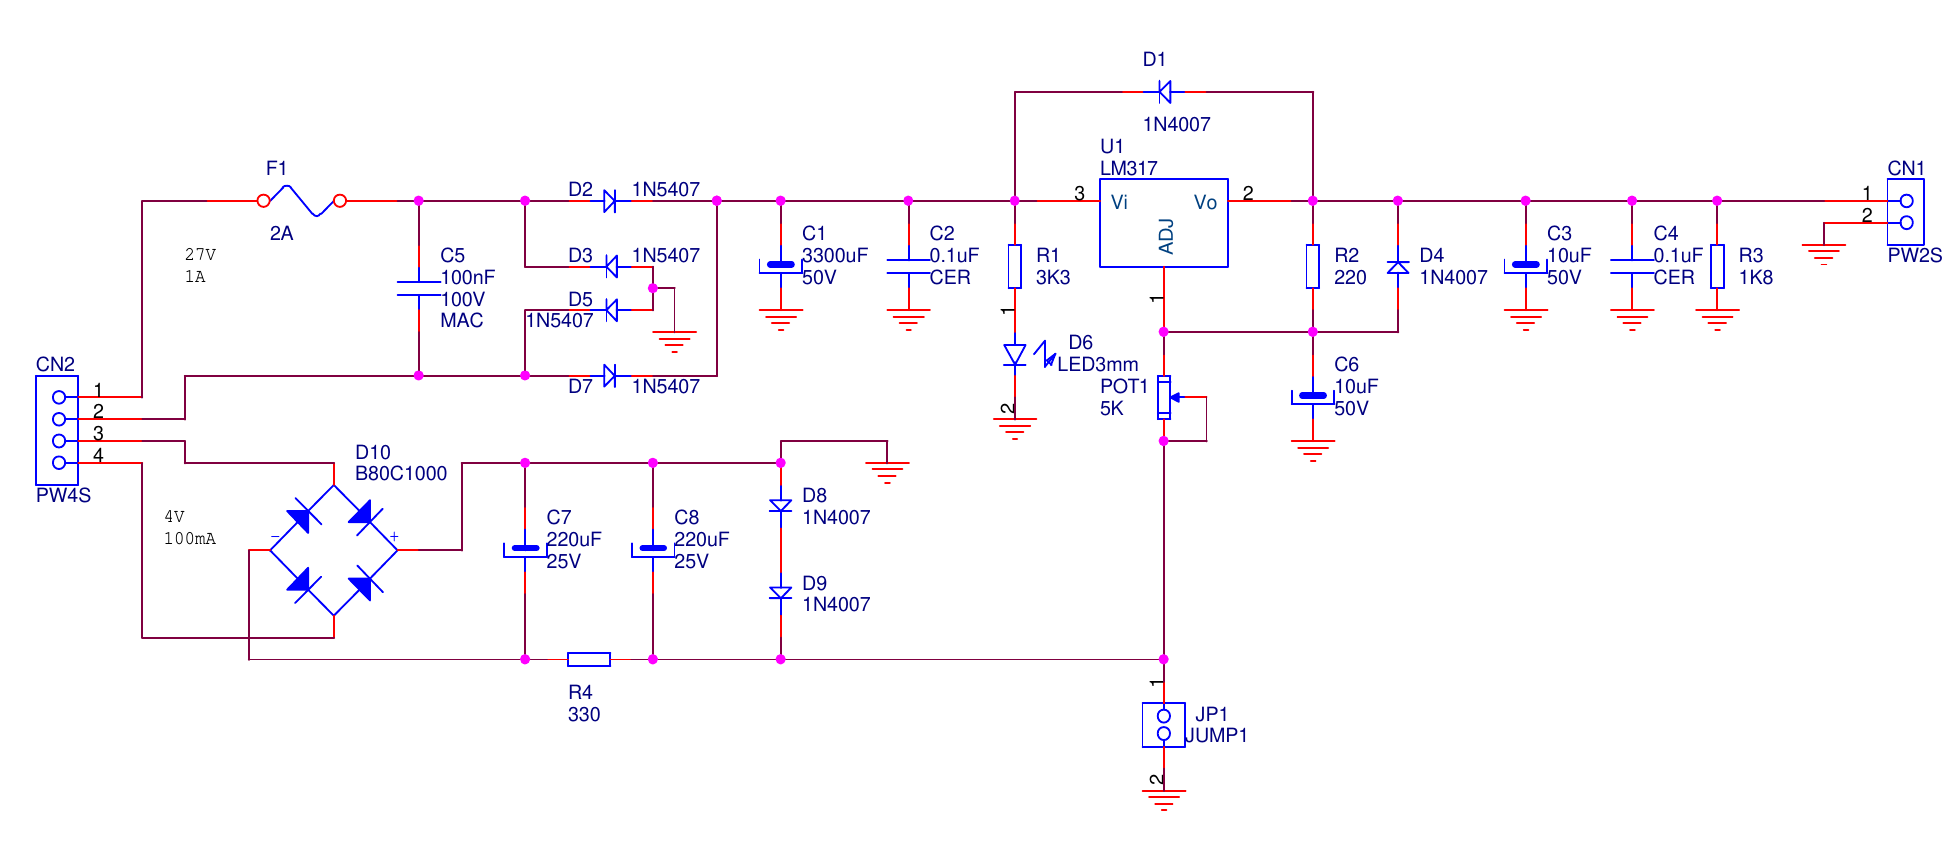
\includegraphics[width=\textwidth]{circuito.png}
    \caption{Esquema de la fuente de alimentación regulada.}
\end{figure}

%--------------------------------
\section{Cálculos teóricos}
%--------------------------------
%\section{Especificaciones del Diseño}
Se realiza el rediseño de la fuente de alimentación regulada propuesta en el \textit{Ejemplo 1} utilizando un nuevo transformador con derivación central (punto medio). Las especificaciones requeridas por la carga se mantienen idénticas:
\begin{itemize}
%    \item Tensión de salida deseada ($V_O$): \SI{9}{\V}
%    \item Corriente máxima en la carga ($I_O$ o $I_L$): \SI{1,5}{\A} 
%    \item Rizado máximo admitido en el PDF ($V_{\text{ripple}}$): $< \SI{1}{\V_{pp}}$
    \item \textbf{Transformador:} \SI{220}{\V} / \SI{12}{\V} + \SI{12}{\V}, \SI{3}{\A} totales (\SI{1.5}{\A} por rama), \SI{50}{\Hz}.
\end{itemize}

La elección de un transformador con derivación central, permite
utilizar el punto bajo (\SI{12}{\V}) u alto (\SI{24}{\V}) según la tensión de salida deseada.
Reducieno de esta forma la caida de tensión en el regulador, y por ende la potencia que debe disipar.

\subsection{Tensión Continua después del Rectificador $V_{DC}$}
La tensión de pico en el capacitor de filtro se calcula como:
\begin{equation}
    V_{DC} = \sqrt{2} \cdot V_{S(\text{rms})} - 2 V_D
\end{equation}
Asumiendo una caída típica en el diodo de silicio de $V_D = \SI{0.7}{\V}$:
\begin{equation}
  V_{DC_{(bajo)}} = \sqrt{2} \cdot \SI{12}{\V} - \SI{1.4}{\V}  = \mathbf{\SI{15.57}{\V}}
\end{equation}
\begin{equation}
    V_{DC_{(alto)}} = \sqrt{2} \cdot \SI{24}{\V} - \SI{1.4}{\V}  = \mathbf{\SI{32.54}{\V}}
\end{equation}

\subsection{Dimensionamiento de los Diodos Rectificadores}

Durante cada semiciclo, solo dos diodos del puente se encuentran conduciendo.

\begin{itemize}
    \item \textbf{Corriente promedio por diodo ($I_{F(AV)}$):} Cada diodo conduce durante la mitad del ciclo completo.
    \begin{equation}
        I_{F(AV)} = \frac{I_O}{2} = \frac{\SI{1500}{\mA}}{2} = \mathbf{\SI{750}{\mA}}
    \end{equation}

  \item \textbf{Corriente eficaz ($I_{S(\text{RMS}})$):}
    \begin{equation}
      I_{S(\text{RMS})} \approx I_O \cdot K \approx \SI{1.5}{\A} \cdot 1.8 = \SI{2.7}{\A}
    \end{equation}

    \item \textbf{Tensión Inversa de Pico ($V_{RRM}$):} En esta topología, el diodo en estado de bloqueo debe soportar el doble de la tensión de pico del devanado secundario:
    \begin{equation}
        V_{RRM} = (\sqrt{2} \cdot V_{S(\text{rms})}) - V_D
    \end{equation}
    \begin{equation}
        V_{RRM} = \SI{32.54}{\V} - \SI{0.7}{\V} = \mathbf{\SI{31.84}{\V}}
    \end{equation}
    \begin{equation}
        V_{RRM} = \SI{15.57}{\V} - \SI{0.7}{\V} = \mathbf{\SI{14.87}{\V}}
    \end{equation}

    \item \textbf{Potencia disipada por diodo ($P_D$):}
    \begin{equation}
        P_D = V_D \cdot I_{F(AV)} = \SI{0.7}{\V} \cdot \SI{0.75}{\A} = \mathbf{\SI{0.525}{\W}}
    \end{equation}
\end{itemize}

%\subsection{Cálculo y Verificación del Capacitor de Filtro ($C_1$)}
%La frecuencia de la señal rectificada en onda completa es el doble de la frecuencia %de red ($f_{\text{ripple}} = 2 \cdot \SI{50}{\Hz} = \SI{100}{\Hz}$). 
%
%\subsubsection{Valor Teórico (Para $V_{\text{ripple}} = \SI{1}{\V_{pp}}$)}
%\begin{equation}
%    C_1 = \frac{I_L}{2 \cdot f_{\text{red}} \cdot V_{\text{ripple}}} = \frac{\SI{1.5}%{\A}}{2 \cdot \SI{50}{\Hz} \cdot \SI{1}{\V}} = \mathbf{\SI{15000}{\micro\F}}
%\end{equation}
%
\subsection{Cálculo de ripple en el filtro}
Para la implementación física del circuito se utiliza un valor comercial estandarizado de \SI{3300}{\micro\F}. Despejando el rizado real obtenido bajo máxima carga resulta:
\begin{equation}
    V_{r(\text{real})} = \frac{I_L}{2 \cdot f_{\text{red}} \cdot C_{\text{real}}} = \frac{\SI{1.5}{\A}}{2 \cdot \SI{50}{\Hz} \cdot \SI{3300}{\micro\F}} \approx \mathbf{\SI{4.54}{\V_{\text{pp}}}}
\end{equation}


\subsection{Resistencias de Programación del LM317 \texorpdfstring{($R_1$ y $R_2$)}{(R1 y R2)}}
La tensión de salida está determinada exclusivamente por la malla de realimentación del regulador. Fijando $R_1 = \SI{220}{\Omega}$ (valor recomendado para garantizar la corriente mínima de carga del integrado):
\begin{equation}
    V_O = V_{\text{ref}} \cdot \left(1 + \frac{R_2}{R_1}\right) + I_{\text{adj}} \cdot R_2
\end{equation}
Despreciando la corriente del terminal de ajuste ($I_{\text{adj}} \approx \SI{50}{\micro\A}$) y tomando $V_{\text{ref}} = \SI{1.25}{\V}$:
\begin{equation}
    \SI{9}{\V} = \SI{1.25}{\V} \cdot \left(1 + \frac{R_2}{\SI{220}{\Omega}}\right) \implies R_2 = \mathbf{\SI{1.36}{\k\Omega}}
\end{equation}

\subsection{Análisis Térmico del Regulador \texorpdfstring{($P_{\text{reg}}$)}{(Preg)}}
La potencia que el LM317 disipa en forma de calor depende directamente de la caída de tensión estática entre su entrada y su salida:
\begin{equation}
    P_{\text{reg}} = (V_{DC} - V_O) \cdot I_O
\end{equation}

Teniendo en cuenta la tensión de salida mínima entregada por el regulador ($V_O = \SI{1.25}{\V}$) y la tensión de salida
del filtro capacitivo ($V_{DC} = \SI{15.57}{\V}$), la potencia disipada por el integrado bajo máxima carga resulta:

\begin{equation}
    P_{\text{reg}} = (\SI{15.57}{\V} - \SI{1.25}{\V}) \cdot \SI{1.5}{\A} = \SI{14.32}{\V} \cdot \SI{1.5}{\A} = \mathbf{\SI{21.48}{\W}}
\end{equation}

Estableciendo una temperatura ambiente $T_a = \SI{25}{\celsius}$ y conociendo que la temperatura máxima de la juntura 
del semiconductor es $T_j = \SI{150}{\celsius}$, calculamos la resistencia térmica total máxima permitida del sistema:

\begin{equation}
    R_{\theta JA(\text{máx})} = \frac{T_j - T_a}{P_{\text{reg}}} = \frac{\SI{150}{\celsius} - \SI{25}{\celsius}}{\SI{21.48}{\W}} \approx \mathbf{\SI{5.819}{\celsius\per\W}}
\end{equation}

\textbf{Conclusión Térmica:} Debido a que la resistencia térmica intrínseca de un encapsulado TO-220 al aire libre ronda
los \SI{50}{\celsius\per\W}, \textbf{es estrictamente obligatorio instalar un disipador térmico} para evitar que actúe
la protección térmica interna del integrado por sobrecalentamiento.


%--------------------------------
\section{Ensayos y mediciones}
%--------------------------------
\subsection{Ensayos sin regulador}

El voltaje de ripple pico-pico en la salida del filtro capacitivo sin regulador de tension, medido con un osciloscopio fue de \SI{2.6}{\V}. Si se aproxima la señal a una onda triangular, el valor eficaz resulta: 

Ver mediciones en el anexo \ref{sec:anexo} \ref{fig:osc}, y \ref{fig:osc1}.

\begin{equation}
    V_{r(\text{rms})} = \frac{V_{r(\text{pp})}}{2\sqrt{3}} = \frac{\SI{2.6}{\V}}{2\sqrt{3}} \approx \mathbf{\SI{0.75}{\V}}
\end{equation}

Para el ensayo del rectificador con filtro se midieron, además, los siguientes valores: $V_{\text{vacio}} = \SI{17.1}{\V}$, $V_{\text{carga}} = \SI{13}{\V}$ y una corriente máxima $I_{\text{máx}} = \SI{1.5}{\A}$. A partir de estos datos, se determina la regulación de voltaje ($RV$) del bloque de filtrado:
\begin{equation}
    RV = \frac{V_{\text{vacio}} - V_{\text{carga}}}{V_{\text{carga}}} \cdot 100\% = \frac{\SI{17.1}{\V} - \SI{13}{\V}}{\SI{13}{\V}} \cdot 100\% = \mathbf{31.54\%}
\end{equation}

El factor de ripple ($FR$) en bornes del capacitor se calcula como:
\begin{equation}
    FR = \frac{V_{r(\text{rms})}}{V_{\text{carga}}} \cdot 100\% = \frac{\SI{0.75}{\V}}{\SI{13}{\V}} \cdot 100\% = \mathbf{5.77\%}
\end{equation}

Para determinar la resistencia interna equivalente de la etapa no regulada en condiciones dinámicas de carga, se evalúa la caída de tensión bajo máxima solicitación de corriente:
\begin{equation}
    R_{\text{int}} = \frac{V_{\text{vacio}} - V_{\text{carga}}}{I_{\text{máx}}} = \frac{\SI{17.1}{\V} - \SI{13}{\V}}{\SI{1.5}{\A}} = \mathbf{2.73\,\Omega}
\end{equation}

\subsection{Ensayos con regulador}
Una vez conectado el regulador integrado LM317, se repitieron los ensayos obteniendo los siguientes valores sobre la carga: $V_{\text{vacio}} = \SI{7.49}{\V}$, $V_{\text{carga}} = \SI{7.33}{\V}$, $V_{r(\text{pp})} = \SI{5}{\mV}$ y $V_{r(\text{rms})} = \SI{1.44}{\mV}$. 

La regulación de voltaje final de la fuente es:
\begin{equation}
    RV = R_{\text{load}} = \frac{V_{\text{vacio}} - V_{\text{carga}}}{V_{\text{carga}}} \cdot 100\% = \frac{\SI{7.49}{\V} - \SI{7.33}{\V}}{\SI{7.33}{\V}} \cdot 100\% = \mathbf{2.18\%}
\end{equation}

Y el factor de ripple remanente en la salida resulta:
\begin{equation}
    FR = \frac{V_{r(\text{rms})}}{V_{\text{carga}}} \cdot 100\% = \frac{\SI{1.44}{\mV}}{\SI{7.33}{\V}} \cdot 100\% = \mathbf{0.0196\%}
\end{equation}

Para evaluar los parámetros de estabilización frente a perturbaciones externas, se procesaron las variaciones medidas en
los extremos de operación de la línea ($\Delta V_i = \SI{24}{\V} - \SI{12}{\V} = \SI{12}{\V}$).
A partir de la máxima variación registrada en la salida: $\Delta V_O = 0.06$ para $V_O = \SI{9.02}{\V}$ y $I_O = \SI{680}{\mA} $.
se calcula la regulación de línea ($R_{\text{línea}}$):

\begin{equation}
    R_{\text{línea}} = \frac{\frac{\Delta V_O}{V_O}}{\Delta V_i} \cdot 100\%/\text{V} = \frac{\frac{\SI{0.06}{\V}}{\SI{9.02}{\V}}}{\SI{12}{\V}} \cdot 100\%/\text{V} \approx \mathbf{0.0462\%/\text{V}}
\end{equation}

Para el análisis térmico del dispositivo se tomaron lecturas con la termocupla de un multímetro digital, registrándose 
una temperatura ambiente $T_{\text{Amb}} = \SI{22}{\celsius}$ y una temperatura sobre la cápsula TO-220 del componente $T_{\text{Carc}} = \SI{51}{\celsius}$. 

Con una caída de tensión estática medida en el regulador de $V_{\text{in}} - V_{\text{out}} = \SI{3.1}{\V}$ a la corriente máxima de ensayo ($I_{\text{máx}} = \SI{1.5}{\A}$), la potencia disipada por el integrado es:
\begin{equation}
    P_{\text{reg}} = (V_{\text{in}} - V_{\text{out}}) \cdot I_{\text{máx}} = \SI{3.1}{\V} \cdot \SI{1.5}{\A} = \mathbf{4.65\,\text{W}}
\end{equation}

A partir de estos valores, la resistencia térmica efectiva entre la carcasa y el ambiente ($R_{\theta CA}$) para la condición de ensayo resulta:

Ver en el anexo \ref{sec:anexo} las mediciones correspondientes \ref{fig:temp}, y \ref{fig:tension-reg}.

\begin{equation}
    R_{\theta CA} = \frac{T_{\text{Carc}} - T_{\text{Amb}}}{P_{\text{reg}}} = \frac{\SI{51}{\celsius} - \SI{22}{\celsius}}{\SI{4.65}{\W}} \approx \SI{6.236}{\celsius\per\W}
\end{equation}

Este valor es significativamente menor al límite máximo calculado en la sección de cálculos teóricos, lo que indica que
el disipador térmico utilizado en el ensayo es adecuado para mantener la temperatura de la juntura del semiconductor
dentro de los límites seguros de operación.


%--------------------------------
\section{Conclusión}
%--------------------------------
A partir de los ensayos experimentales realizados, se verificó el correcto funcionamiento de las distintas etapas de la
fuente de alimentación regulada.

El bloque de filtrado capacitivo, utilizando un componente comercial de \SI{3300}{\micro\F}, exhibió un factor de ripple
inicial del \textbf{5.77\%} bajo condiciones de máxima carga (\SI{1.5}{\A}).

Tras la incorporación del integrado LM317, el factor de ripple
residual en la salida se redujo drásticamente a un valor despreciable de \textbf{0.0196\%}, lo que representa una atenuación
de más de \SI{54}{\dB}. Los parámetros de regulación de línea (\SI{0.0462}{\%/\text{V}}) y de carga (\SI{2.183}{\%}) ratifican
la estabilidad de la tensión suministrada frente a fluctuaciones en la red o demandas dinámicas de corriente. 

Finalmente, el análisis térmico determinó una resistencia de carcasa a ambiente de \SI{6.236}{\celsius\per\W}. Valida la
elección del disipador térmico utilizado, asegurando que la temperatura de la juntura del LM317 permanezca dentro de los
límites seguros de operación.

%--------------------------------
\section{Anexo} \label{sec:anexo}
%--------------------------------
\begin{figure}[H]
    \centering
    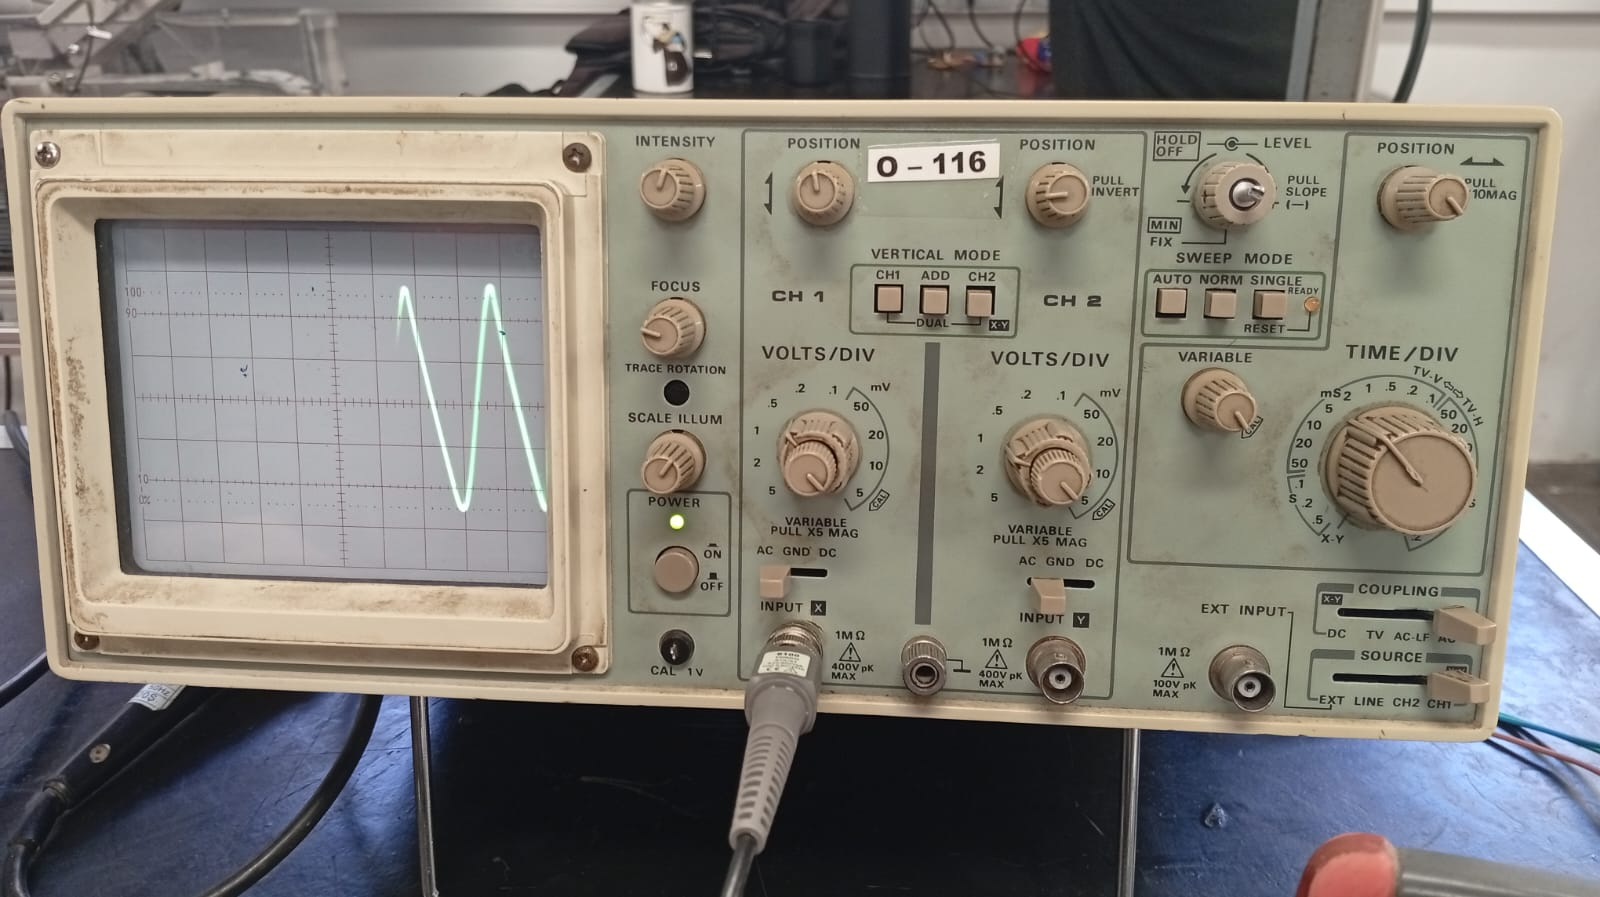
\includegraphics[width=0.6\textwidth]{osc.jpeg}
    \caption{Osciloscopio utilizado}
    \label{fig:osc}
\end{figure}

\begin{figure}[H]
    \centering
    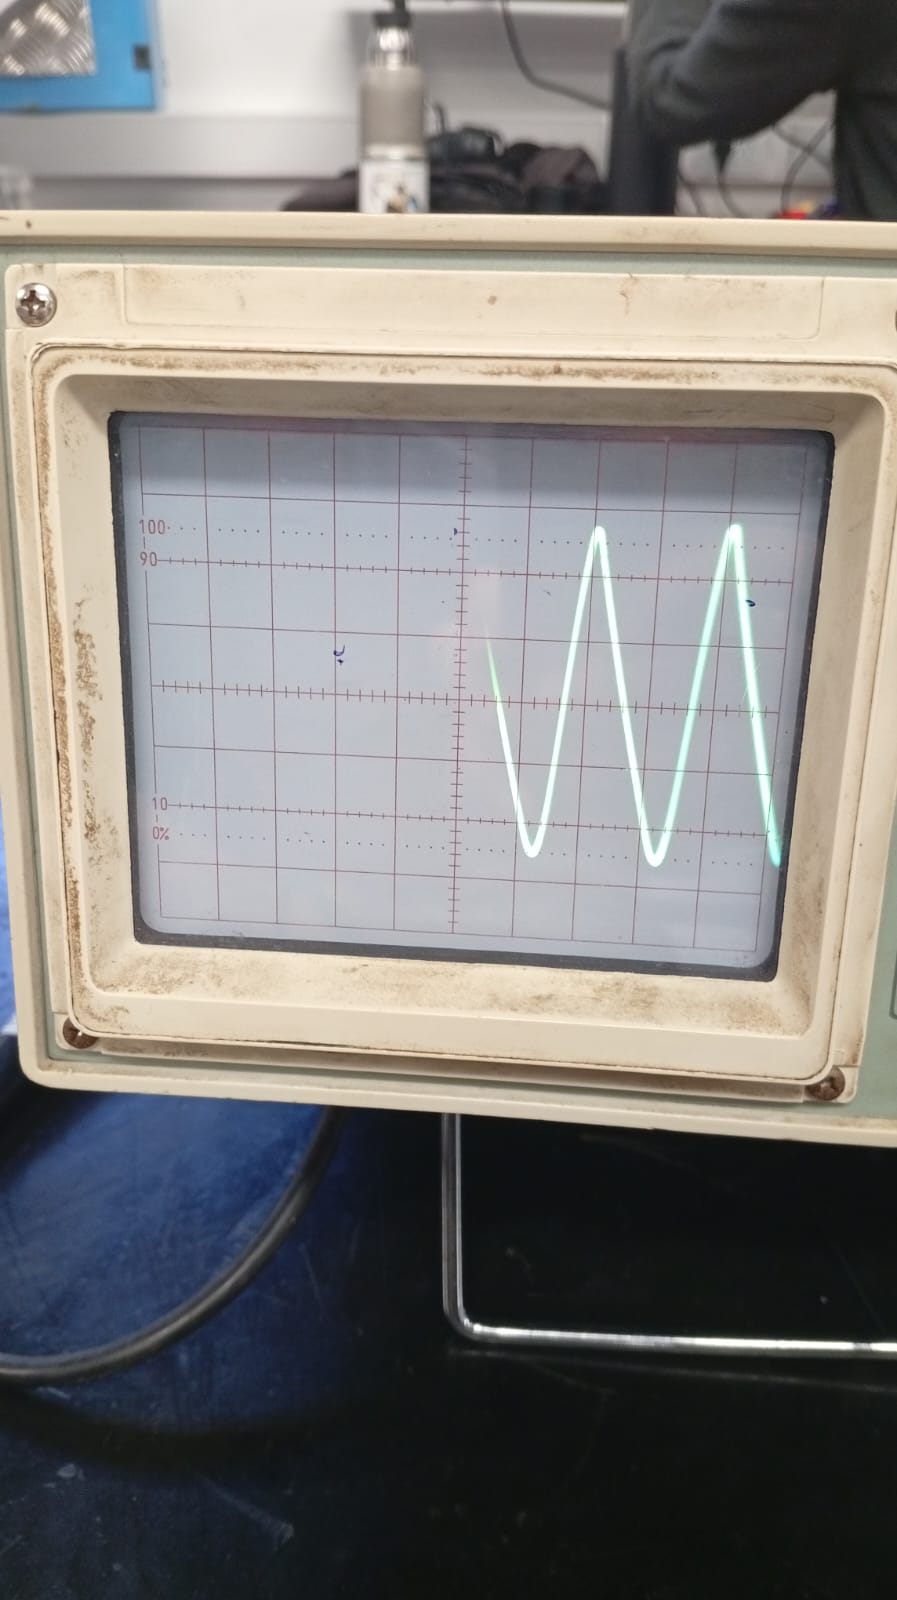
\includegraphics[width=0.5\textwidth]{osc1.jpeg}
    \caption{Función en osciloscopio}
    \label{fig:osc1}
\end{figure}

\begin{figure}[H]
    \centering
    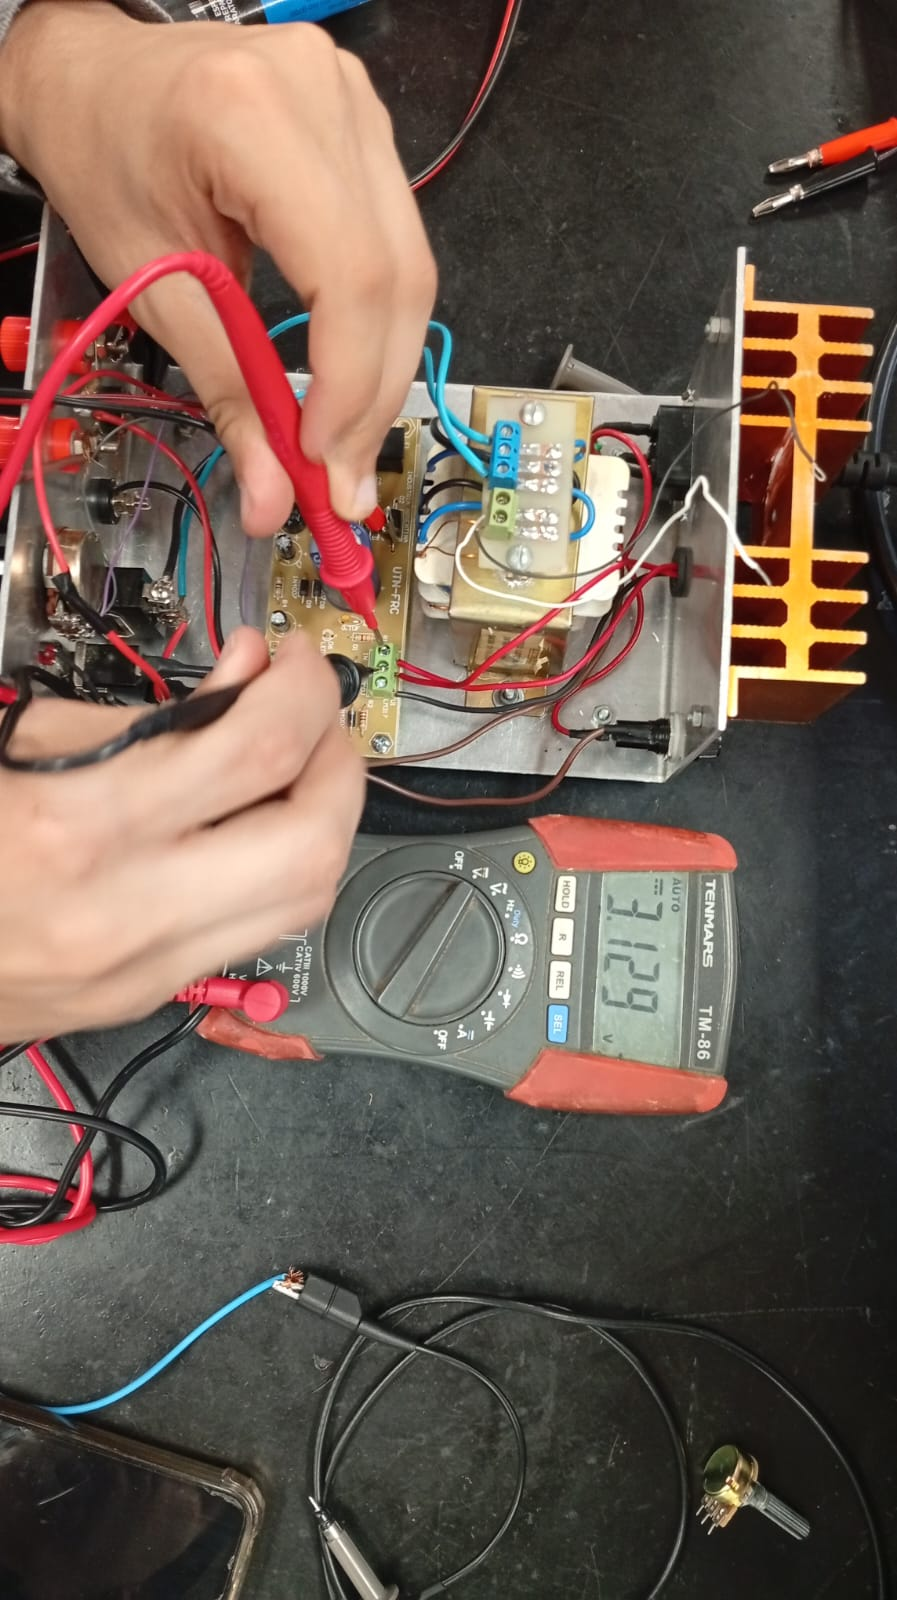
\includegraphics[width=0.6\textwidth]{med.jpeg}
    \caption{Caida de tensión en el regulador}
    \label{fig:tension-reg}
\end{figure}

\begin{figure}[H]
    \centering
    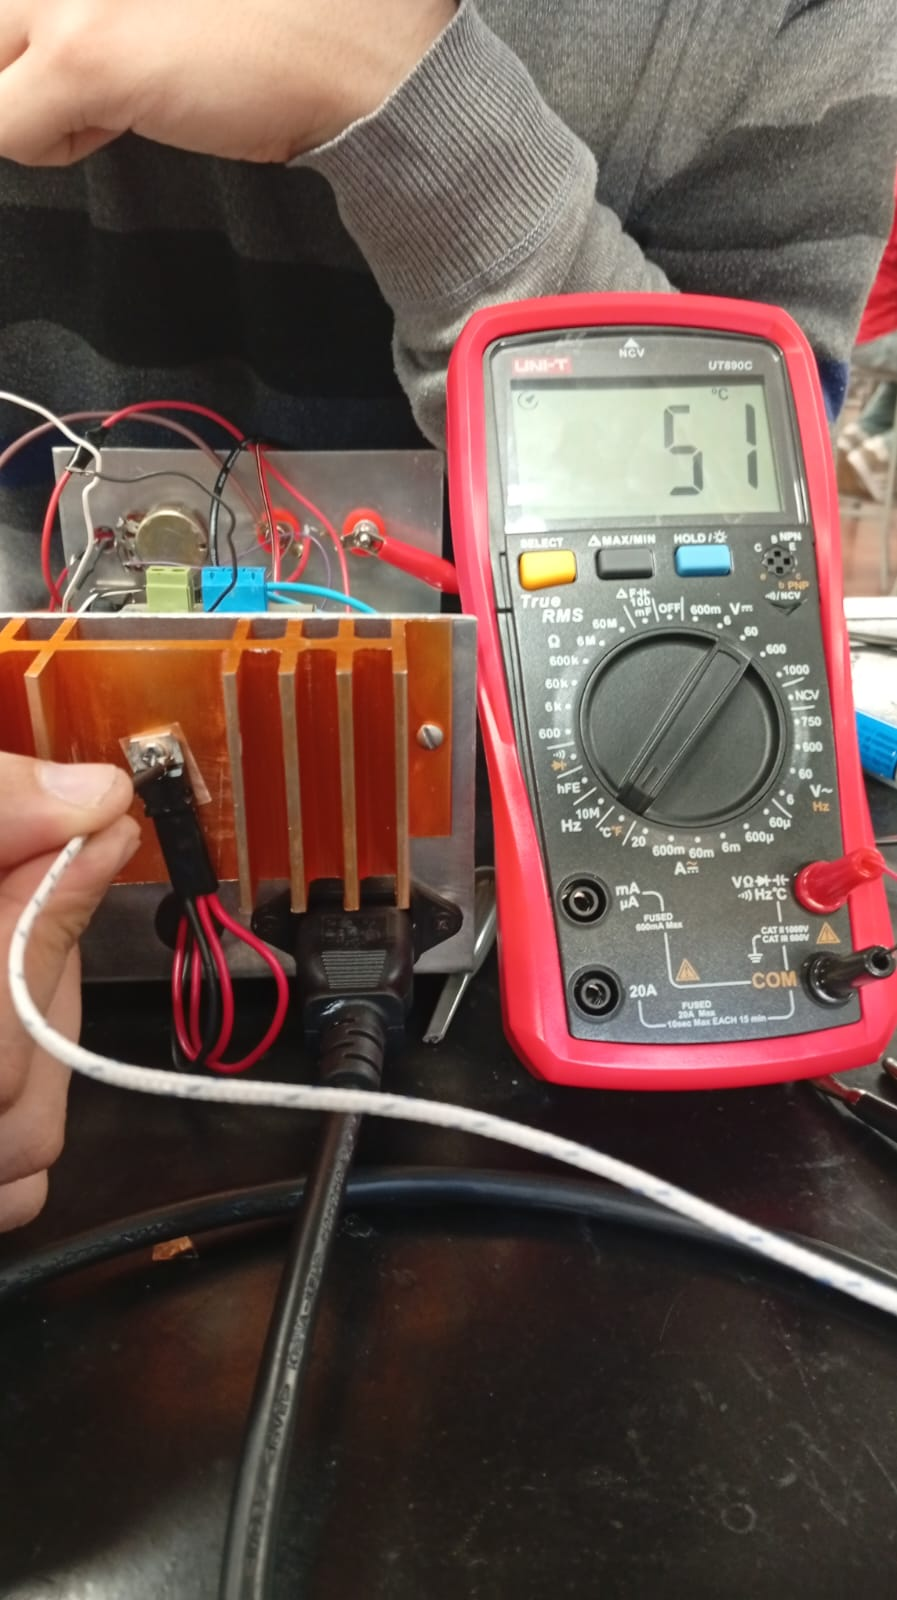
\includegraphics[width=0.6\textwidth]{temp.jpeg}
    \caption{Medición de temperatura}
    \label{fig:temp}
\end{figure}

%--------------------------------


\end{document}